\section*{MUESTRA}\label{sec:muestra}

\addcontentsline{toc}{section}{MUESTRA}
\begin{figure}[ht]
    \centering
    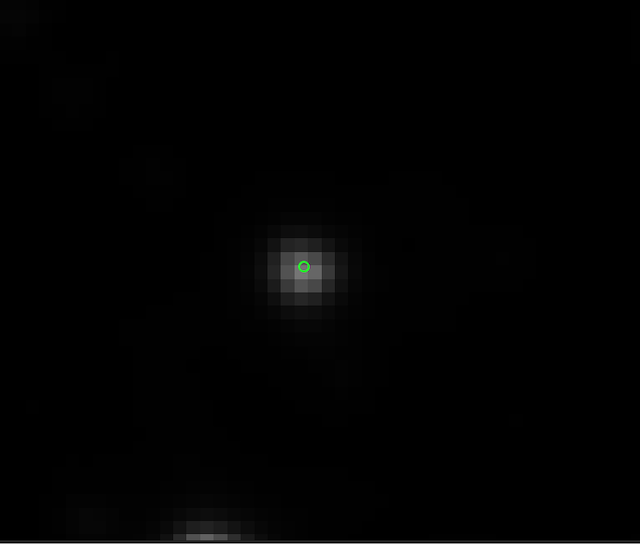
\includegraphics[scale=0.35]{Imagenes/Rudik-1.png}
    \caption{IGRF17451}
    \label{fig:estrella-rudik}
\end{figure}
\begin{figure}[ht]
    \centering
    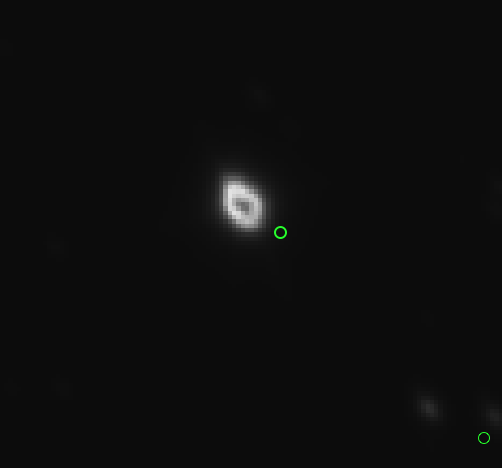
\includegraphics[scale=0.4]{Imagenes/Baptiste-1.png}
    \caption{MAXIJ1543}
    \label{fig:estrella-bapt}
\end{figure}

% Please add the following required packages to your document preamble:
% \usepackage{booktabs}
\begin{table*}[t]
\caption{}
\label{tab:estrellas}
\begin{tabular}{@{}lllllllllll@{}}
\toprule
Imagen     & \begin{tabular}[c]{@{}l@{}}Coordenadas \\ ecuatoriales\end{tabular}       & Color   & \begin{tabular}[c]{@{}l@{}}Tempe-\\ ratura\end{tabular} & \begin{tabular}[c]{@{}l@{}}Distancia\\ (m)\end{tabular} & \begin{tabular}[c]{@{}l@{}}Lumino-\\ sidad (W)\end{tabular} & \begin{tabular}[c]{@{}l@{}}Flujo     \\ (W/m²)\end{tabular} & Tamaño & \begin{tabular}[c]{@{}l@{}}Tipo \\ Espectral\end{tabular} & \begin{tabular}[c]{@{}l@{}}Clase \\ Lumi-\\ nosidad\end{tabular} & \begin{tabular}[c]{@{}l@{}}Posición \\ (HR)\end{tabular} \\ \midrule
IGRFJ17451 & \begin{tabular}[c]{@{}l@{}}Ra: 266.232544\\ Dec: -30.390377\end{tabular}  & 5.06E-7 & 5778                                                    & 3.112 E19                                               & 0.994                                                       & 3.1 E-14                                                    & 0.99   & G2                                                        & V                                                                & MS                                                       \\
MAXIJ1543  & \begin{tabular}[c]{@{}l@{}}Ra:  235.955621\\ Dec: -56.440075\end{tabular} & 3.62E-7 & 8000                                                    & 1.97E19                                                 & 2.59                                                        & 2.0E-13                                                     & 0.8385 & K II                                                        & V                                                                & MS                                                       \\ \bottomrule
\end{tabular}
\end{table*}


\begin{table}[t]
\caption{}
\label{tab:estrellas2}
\begin{tabular}{@{}lllll@{}}
\toprule
Imagen     & Instrumento & Fecha de observación & Filtro &  \\ \midrule
IGRFJ17451 & LIRIS       & 9 de abril 2015      & $K_s$   &  \\
MAXIJ1543  & HAWK-I      & 10 de abril 2018     & H      &  \\ \bottomrule
\end{tabular}
\end{table}